\section{Figuras e tabelas}
%------------------------------------------
%----------------FIGURE--------------------
\begin{figure*}[ht!]
\centering
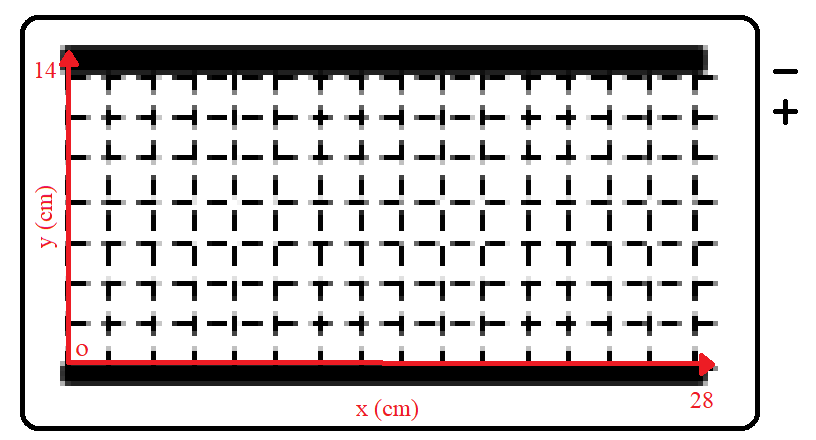
\includegraphics[width = 9 cm]{figuras/fig1.png}
\caption{\small{Posicionamento do sistema de coordenadas $(x,y)$ no esquema experimental.}}
\label{fig:1}
\end{figure*}
%------------------------------------------
%------------------------------------------


%------------------------------------------
%----------------FIGURE--------------------
\begin{figure*}[ht!]
\centering
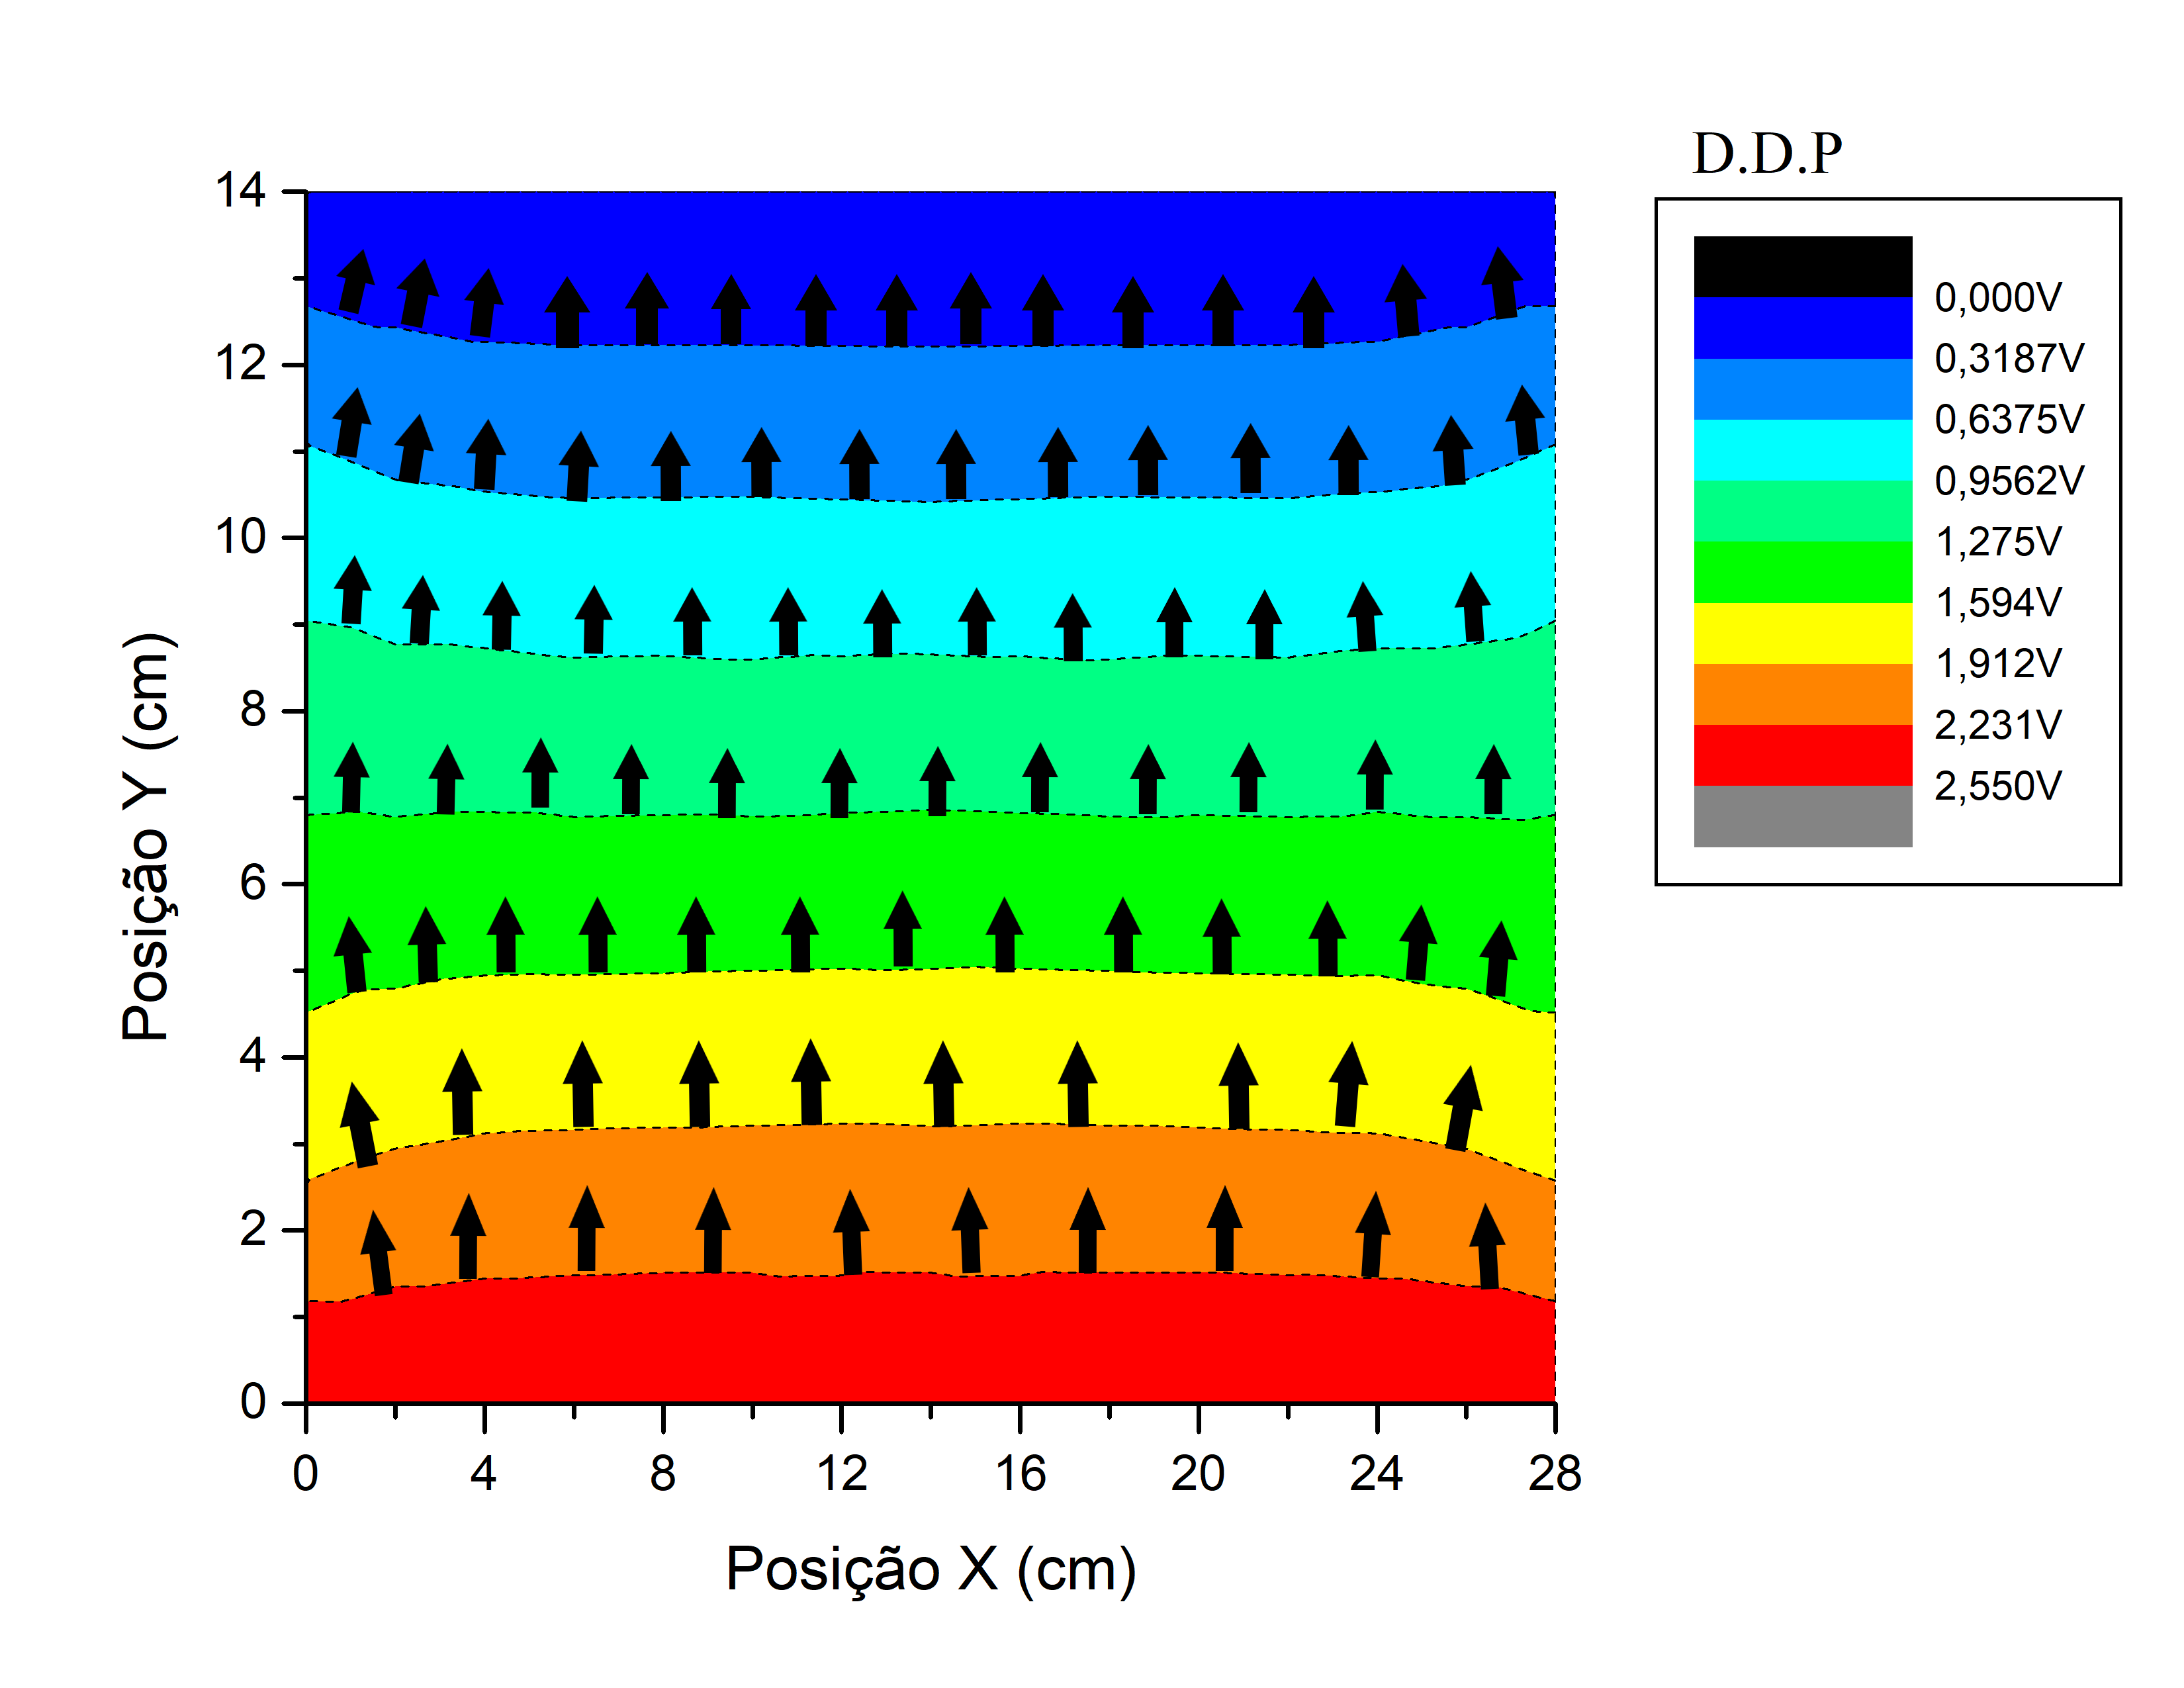
\includegraphics[width = 9 cm]{figuras/Graph5.png}
\caption{\small{Gráfico do potencial e do sentido do campo elétrico no plano com linhas equipotenciais em pontilhado do caso Figura 2(a).}}
\label{fig:2}
\end{figure*}
%------------------------------------------
%------------------------------------------

%------------------------------------------
%----------------FIGURE--------------------
\begin{figure*}[ht!]
\centering
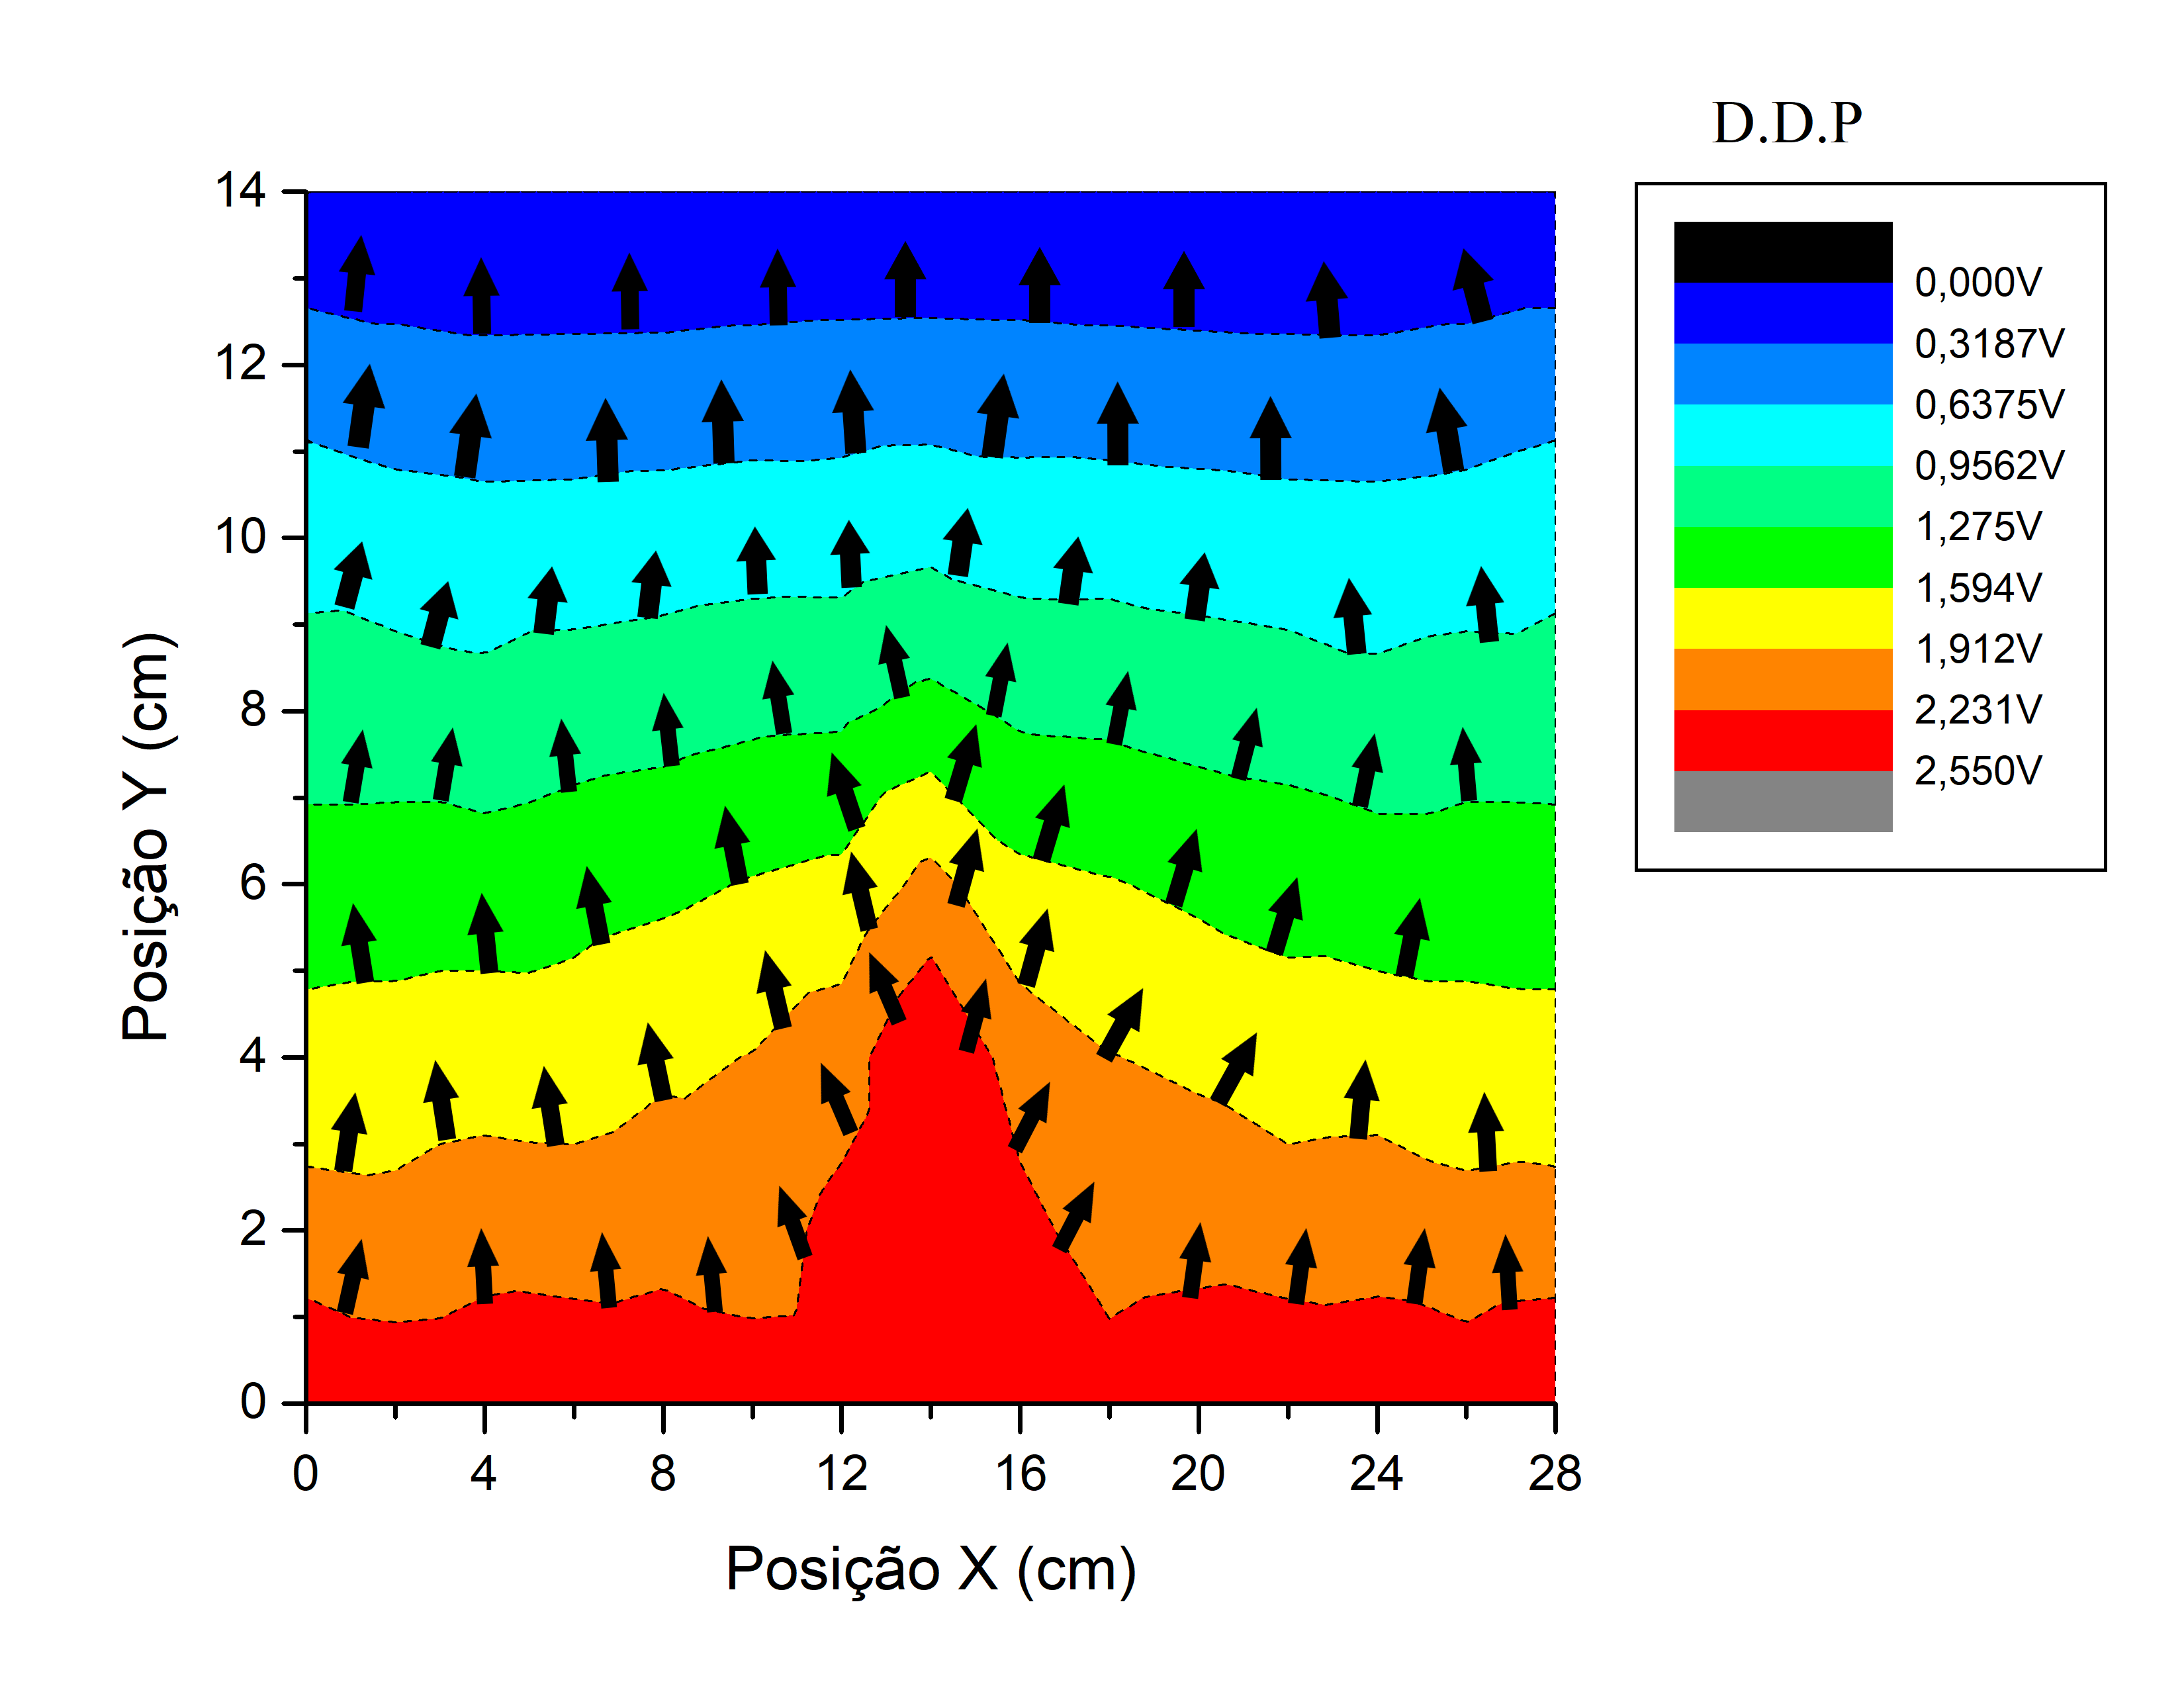
\includegraphics[width = 9 cm]{figuras/Graph4.png}
\caption{\small{Gráfico do potencial e do sentido do campo elétrico no plano com linhas equipotenciais em pontilhado do caso Figura 2(b).}}
\label{fig:3}
\end{figure*}
%------------------------------------------
%------------------------------------------

%------------------------------------------
%----------------FIGURE--------------------
\begin{figure*}[ht!]
\centering
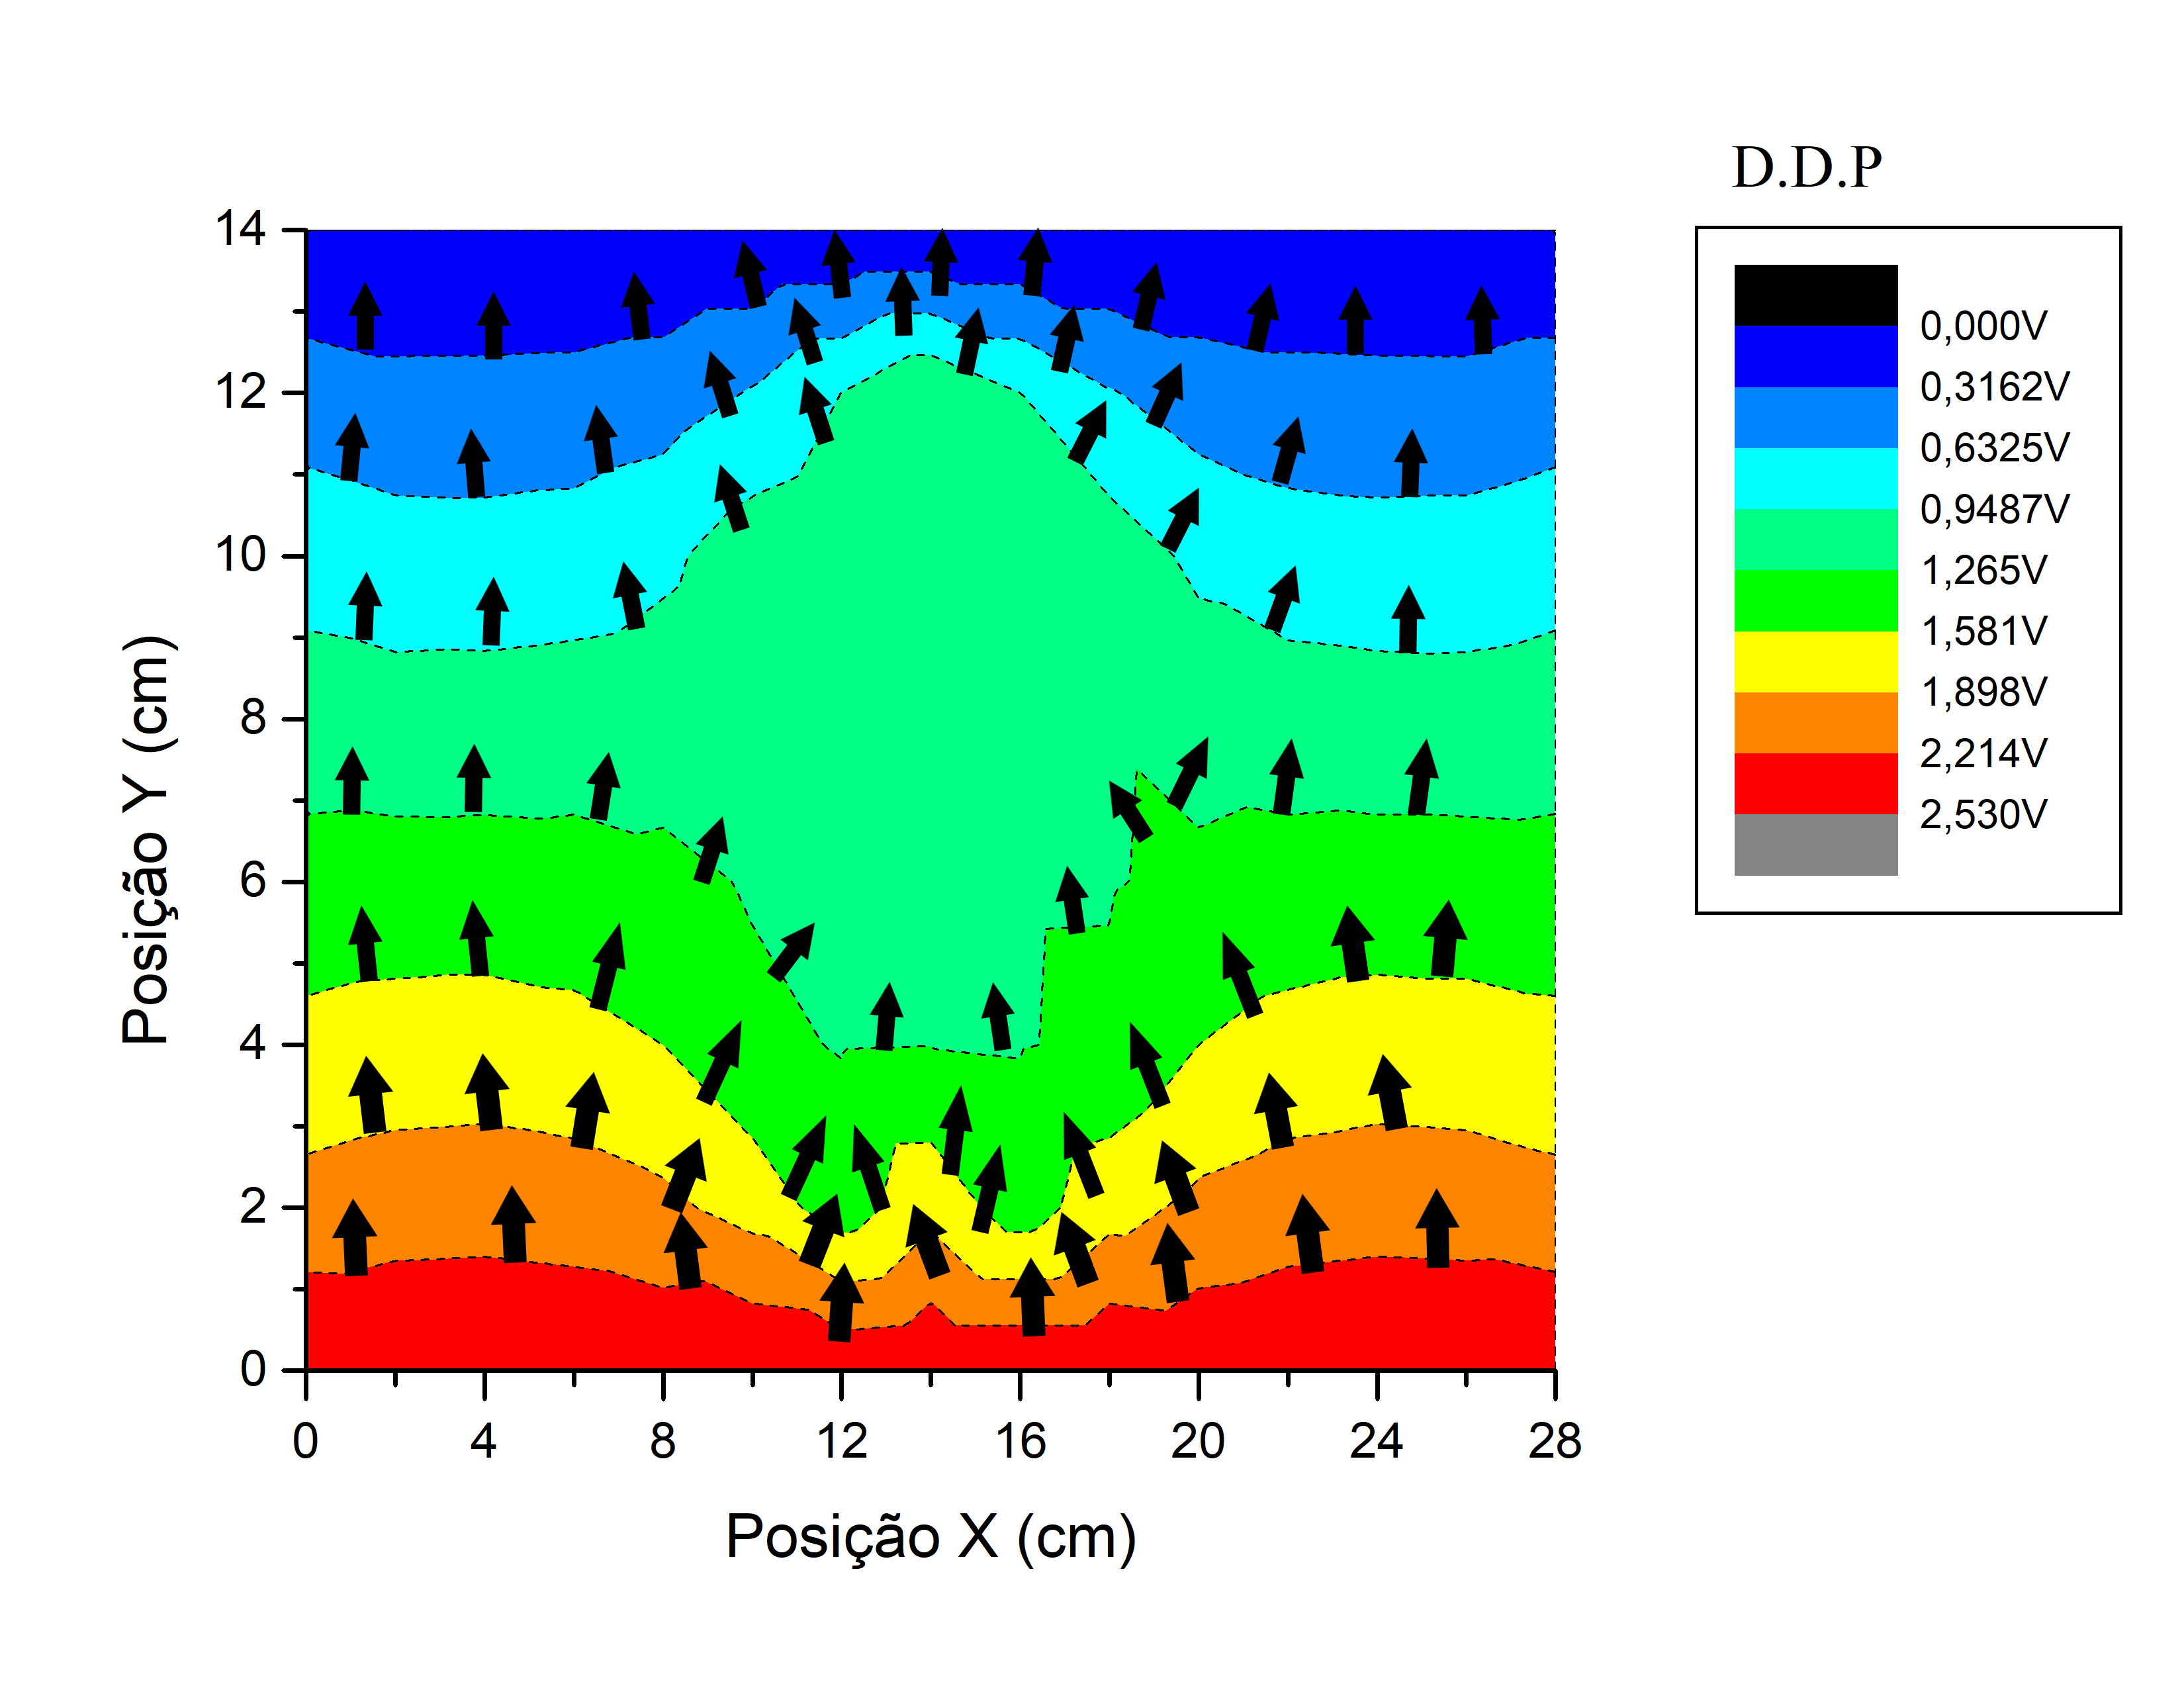
\includegraphics[width = 9 cm]{figuras/Graph1.png}
\caption{\small{Gráfico do potencial e do sentido do campo elétrico no plano com linhas equipotenciais em pontilhado do caso Figura 2(c).}}
\label{fig:4}
\end{figure*}

%------------------------------------------
%----------------FIGURE--------------------
\begin{figure*}[ht!]
\centering
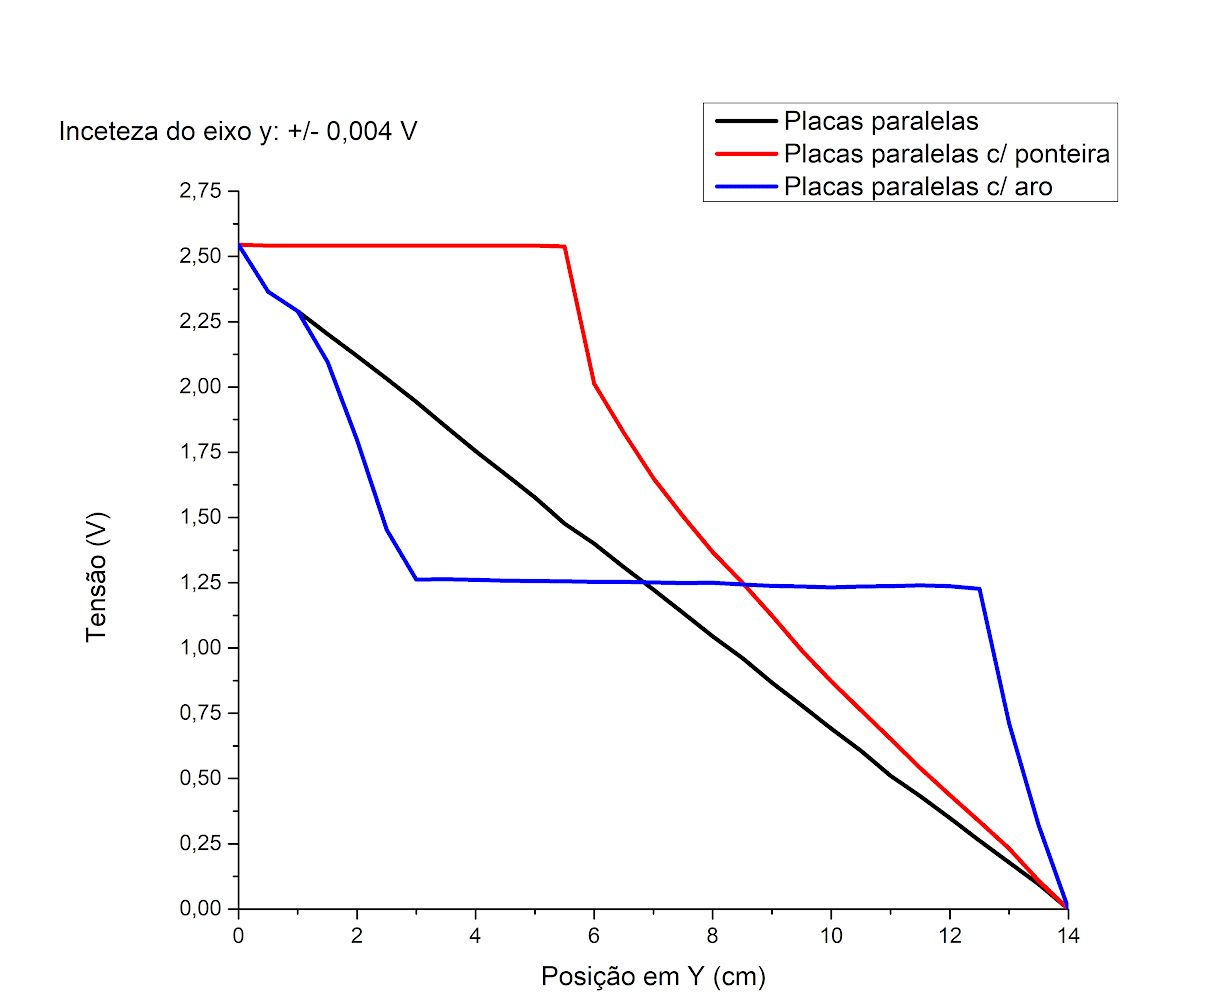
\includegraphics[width = 9 cm]{figuras/Graph6.png}
\caption{\small{Gráfico do potencial no eixo de simetria de cada uma das configurações 2(a), 2(b) e 2(c); incerteza não é visível no gráfico.}}
\label{fig:8}
\end{figure*}
%------------------------------------------
%------------------------------------------

\begin{table}[ht!]
\center
\begin{tabular}{|l|l|l|l|}
\hline
Caso & Figura 2(a) & Figura 2(b) & Figura 2(c) \\ \hline
Módulo do campo elétrico (N/C) &17.60$\pm 0.01$     & 29.20  $\pm 0.01$     & 0.40 $\pm 0.01$
\\ \hline
\end{tabular}
\caption{Módulo do campo elétrico no centro de cada caso.}
\label{tab:1}
\end{table}

Dados coletados podem ser vistos em: \url{https://docs.google.com/spreadsheets/u/1/d/1pe6sFZzzPrPHZEJ3koOhgrh1rRJFGEONfTtdWh-XQDs/edit?usp=sharing}.
%------------------------------------------
%------------------------------------------

